 %%%%%%%%%%%%%%%%%%%%%%%%%%%%%%%%%%%%%%%%%%%%%%%%%%%%%%%%%%%%
%% This Beamer template was created by Cameron Bracken.
%% Anyone can freely use or modify it for any purpose
%% without attribution.
%%
%% Last Modified: January 9, 2009
%%
\documentclass[xcolor=x11names,compress,t]{beamer}
\usepackage{algorithm,algorithmic, color, tikz}
%% General document %%%%%%%%%%%%%%%%%%%%%%%%%%%%%%%%%
%%\usepackage{tikz}

\usepackage{array}

\usepackage{amssymb}% http://ctan.org/pkg/amssymb
\usepackage{pifont}% http://ctan.org/pkg/pifont
\newcommand{\cmark}{{\color{blue}\selectfont \ding{51}} \vspace{.2 cm}}%
\newcommand{\xmark}{{\color{red}\selectfont \ding{55}} \vspace{.18 cm}}%

\usepackage[makeroom]{cancel}
\usepackage{verbatim}
\usetikzlibrary{arrows,shapes,arrows.meta,calc}

\newcommand{\even}[0]{\text{Even}}
\newcommand{\odd}[0]{\text{Odd}}
\newcommand{\negg}[0]{\text{Neg}}
\newcommand{\poss}[0]{\text{Pos}}

\newcommand{\match}[3]{
\item {\textbf{#1}\newline Appears #2 times. Example match: \\\{#3\} \newline}
}
\newcommand{\matchone}[2]{
\item {\textbf{#1}\newline Match: \{#2\} \newline}
}

%\usepackage{silence}
\usepackage{graphicx}
\usepackage{epstopdf}
\usepackage{ragged2e}
\usepackage{soul}
%\usepackage[all, cmtip]{xy}
%\usepackage{tikz}
%\usetikzlibrary{decorations.fractals}
%%%%%%%%%%%%%%%%%%%%%%%%%%%%%%%%%%%%%%%%%%%%%%%%%%%%%%

\newcommand{\g}{\mathfrak{g}}
\newcommand{\CC}{\mathbb{C}}
\newcommand{\ot}{\otimes}
\newcommand{\id}{\operatorname{id}}
\newcommand{\bt}{\boxtimes}
\newcommand{\ZZ}{\mathbb{Z}}
\newcommand{\cO}{\mathcal{O}}
\newcommand{\cD}{\mathcal{D}}
\newcommand{\dd}{\mathbf{d}}
\newcommand{\ev}{\operatorname{ev}}

\def\HH{\hbox{${\mathcal H}$\kern-5.2pt${\mathcal H}$}}
\newcommand{\Mat}{\operatorname{Mat}}
\setbeamertemplate{navigation symbols}{}
\setbeamercolor{block title}{bg=blue!40}
\setbeamercolor{block body}{bg=blue!20}

%\usepackage{refcheck}
%\ErrorFilter{xy}{No room for a new}
%\usepackage[all,cmtip,curve, knot,frame]{xy}
\usepackage{amssymb}
\usepackage{amsfonts}
\usepackage{latexsym}
\usetikzlibrary{matrix}
\usepackage{mathabx}
%% Beamer Layout %%%%%%%%%%%%%%%%%%%%%%%%%%%%%%%%%%

\useoutertheme[subsection=false,shadow]{miniframes}
\useinnertheme{default}
\usefonttheme{serif}
\usepackage{palatino}
\setbeamerfont{title like}{shape=\scshape}
\setbeamerfont{frametitle}{shape=\scshape}
\setbeamercolor*{lower separation line head}{bg=DeepSkyBlue4}
\setbeamercolor*{normal text}{fg=black,bg=white}
\setbeamercolor*{alerted text}{fg=red}
\setbeamercolor*{example text}{fg=black}
\setbeamercolor*{structure}{fg=black}
\setbeamercolor*{palette tertiary}{fg=black,bg=black!10}
\setbeamercolor*{palette quaternary}{fg=black,bg=black!10}
\renewcommand{\(}{\begin{columns}}
\renewcommand{\)}{\end{columns}}
\newcommand{\<}[1]{\begin{column}{#1}}
\renewcommand{\>}{\end{column}}
\newcommand{\rot}{\operatorname*{rot}}
\newtheorem{remark}{Remark}
\newtheorem{thm}{Theorem}
\newtheorem{defn}{Definition}
\newtheorem{lem}{Lemma}
\newtheorem{cor}{Corollary}
\newtheorem{conj}{Conjecture}
\newtheorem{problemstatement}{Problem}
\usepackage{hanging}
\setbeamertemplate{footnote}{\hangpara{2em}{1}\makebox[2em][l]{\insertfootnotemark}\scriptsize\insertfootnotetext\par}

\def \av {\text{AV}}
\newcommand{\bb}[1]{\color{blue} #1}
\newcommand{\rr}[1]{\color{red} #1}
\newcommand{\gr}[1]{\color{gray} #1}
\newcommand{\bin}[0]{\text{Bin}}
\newcommand{\ed}[0]{\operatorname{ed}}
\newcommand{\xpivot}[0]{\text{xpivot}}
\newcommand{\ypivot}[0]{\text{ypivot}}
\newcommand{\ypivotopt}[0]{\text{ypivot}_{\text{opt}}}
\def \av {\text{AV}}
\renewcommand{\epsilon}{\varepsilon}
%%%%%%%%%%%%%%%%%%%%%%%%%%%%%%%%%%%%%%%%%%%%%%%%%%
\usepackage[utf8]{inputenc}
\usepackage[T1]{fontenc}
\usepackage{soul}

% ---------- TikZ helpers for Two-World slides (improved) ----------
% Dimensions (scaled down for better fit)
\def\binw{0.9}
\def\binh{0.3}
\def\bingap{0.35}
\def\biny{-1.9}
\def\ballsize{0.52cm}
\def\ballspacing{0.625}

% World positions so that the bin groups are centered in the left/right halves
% of the slide, using Beamer's default \paperwidth = 12.8cm.
% We model the slide width as [-6.4,6.4] in our x-coordinates (1 unit = 1cm),
% so the 25% and 75% positions are at x = -3.2 and x = +3.2.
% Each group has width W = 4*(\binw) + 3*(\bingap) = 4.65, so the starting
% x-positions are center - W/2.
\def\xL{-5.525} % left world: [-5.525, -0.875], centered at -3.2
\def\xR{0.875}  % right world: [0.875, 5.525], centered at +3.2

\newcommand{\DrawBinsAt}[1]{% xstart
  \foreach \i in {0,1,2,3}{
    \pgfmathsetmacro{\x}{#1 + \i*(\binw+\bingap)}
    % Draw bin as open-top container with slight rounded corners
    \draw[line width=1pt, black!80] (\x,\biny) -- (\x,\binh);
    \draw[line width=1pt, black!80] ({\x+\binw},\biny) -- ({\x+\binw},\binh);
    \draw[line width=1pt, black!80] (\x,\biny) -- ({\x+\binw},\biny);
  }
}

\newcommand{\BallInBin}[5]{% xstart, bin(1-4), level(1..), tikz style, text
  \pgfmathsetmacro{\xx}{#1+(#2-1)*(\binw+\bingap)+0.5*\binw}
  \pgfmathsetmacro{\yy}{\biny+0.35+(#3-1)*\ballspacing}
  \node[circle, draw, minimum size=\ballsize, inner sep=0pt, line width=0.8pt, fill=black!15, #4] at (\xx,\yy) {\scriptsize #5};
}

\newcommand{\BinTop}[3]{% xstart, bin(1-4), name
  \pgfmathsetmacro{\tx}{#1+(#2-1)*(\binw+\bingap)+0.5*\binw}
  \coordinate (#3) at (\tx,{\binh-0.1});
}

\newcommand{\TopSeq}{}% Now integrated into TwoWorldFigure

\newcommand{\TwoWorldFigure}[2]{% extra tikz for world0 balls, world1 balls
  % Center the entire picture with respect to the full slide width (\paperwidth).
  % Shift left by half of (paperwidth - textwidth) to compensate for the theme's
  % right-shift of the text area.
  \noindent\hspace*{-0.5\dimexpr\paperwidth-\textwidth\relax}%
  \makebox[\paperwidth][c]{%
  \begin{tikzpicture}[x=1cm,y=1cm,scale=0.95]
    % Fix the bounding box to be symmetric around x=0 with total width equal
    % to Beamer's default \paperwidth = 12.8cm, i.e., [-6.4,6.4].
    \path[use as bounding box] (-6.4,-3.0) rectangle (6.4,3.0);
    % Debug guide (commented out):
    % \draw[dashed, very thin, gray!50] (-6.4,-3.0) rectangle (6.4,3.0);
    % separator line
    \draw[dash pattern=on 4pt off 3pt, line width=0.8pt, black!35] (0,-2.8) -- (0,2.8);

    % bins for both worlds
    \DrawBinsAt{\xL}
    \DrawBinsAt{\xR}

    % S_0 and S_1 labels removed for cleaner look - the animation shows insertions step by step
    % \node[font=\small, anchor=north] at ({\xL+1.5*(\binw+\bingap)+0.5*\binw},2.8) {$S_0 = x_1,x_2,x_3,x_4,\ldots$};
    % \node[font=\small, anchor=north] at ({\xR+1.5*(\binw+\bingap)+0.5*\binw},2.8) {$S_1 = x_1,x_2,x_3,x_4,{\color{blue}x^{\star}},\ldots$};

    % world labels below bins
    \node[font=\normalsize\bfseries] at ({\xL+1.5*(\binw+\bingap)+0.5*\binw},-2.45) {World 0};
    \node[font=\normalsize\bfseries] at ({\xR+1.5*(\binw+\bingap)+0.5*\binw},-2.45) {World 1};

    % bin-top coords for arrows
    \foreach \b in {1,2,3,4}{
      \BinTop{\xL}{\b}{LT\b}
      \BinTop{\xR}{\b}{RT\b}
    }

    % balls (passed in via arguments)
    #1
    #2
  \end{tikzpicture}
  }%
  \vspace{-2mm}
}

% styles for Two-World slides (improved colors)
\tikzset{
  RedBallStyle/.style={draw=red!80!black, fill=red!20, text=red!80!black, line width=0.9pt},
  BlueOutlineStyle/.style={draw=blue!80!black, fill=blue!10, text=blue!80!black, line width=0.9pt},
  BlueFillStyle/.style={fill=blue!70, draw=blue!90!black, text=white, line width=0.9pt}
}

\begin{document}

\begin{frame}
  \title{History-Independent Load Balancing}  
  
  \author{
    Michael A.~Bender\inst{1} \and
    Bill Kuszmaul\inst{2} \and
    Elaine Shi\inst{2} \and
    \textbf{Rose Silver\inst{2}}
  }
  \institute{
    \inst{1} Stony Brook University \and
    \inst{2} Carnegie Mellon University
  }
  \date{}
  \maketitle
\end{frame}


\begin{frame}{History Independent Data Structures}

\vspace{2 cm}

\textbf{History Independence: }``If an adversary were to see the state of the data structure,
they would learn only the current set of elements, and nothing else about the history of past operations.''\\

\vspace{.2 cm}

\hfill {\tiny \color{blue} [Micciancio '97], [Naor, Teague '01]}\\

\vspace{ 1cm} 

\end{frame}



\begin{frame}{History vs Content}

\(
\<{0.35\textwidth}
  \begin{center}
  \includegraphics[height = 8 cm]{./contacts.jpg}
  \end{center}
\>
\<{0.65\textwidth}
\begin{itemize}
\item If someone hacks my phone, they can learn my contacts list. \pause

\vspace{0.5 cm}

\item But can they learn who my contacts were in the past? \pause

\vspace{0.5 cm}
  
\item What about the order in which contacts were added? \pause

\vspace{0.5 cm}

\item A history independent data structure protects this kind of information.
\end{itemize}
\>
\)
\end{frame}



\begin{frame}{History Independent is a Security Guarantee}

\vspace{1 cm}

\textbf{History Independence: }``If an adversary were to see the state of the data structure,
they would learn only the current set of elements, and nothing else about the history of past operations.''\\ 

\vspace{.2 cm}

\hfill {\tiny \color{blue} [Micciancio '97], [Naor, Teague '01]}\\ \pause

\vspace{0.4 cm} 

\textbf{Lost of successes: } Hash tables, trees, memory allocation, PMAs, graph algorithms, B-trees, cache-oblivious data structures...
{\tiny \color{blue} [Micciancio '97], [Naor, Teague '01], [Buchbinder, Petrank '03], [Molnar, Kohno, Sastry, Wagner '06], [Blelloch, Golovin '07], [Moran, Naor, Segev '07] [Naor, Segev, Wieder '08], [Golovin '08 '09 '10], [Tzouramanis '12], [Bajaj, Sion '13] [Bajaj, Chakrabati, Sion '15], [Roche, Aviv, Choi '15], [Bender, Berry, Johnson, Kroeger, McCauley, Phillips, Simon, Singh, Zage '16], ...} \pause

\vspace{.3 cm}

\textbf{But... some very basic questions also remain open.}

\end{frame}

\begin{frame}{Two-Choice Load Balancing}

\begin{center}
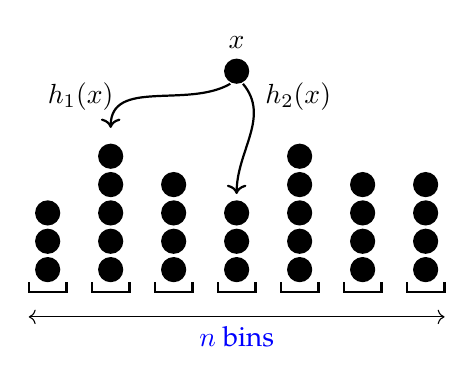
\begin{tikzpicture}[scale=0.8]
  % Define bin dimensions
  \def\binwidth{0.6}
  \def\binheight{2.5}
  \def\ballradius{0.2}
  \def\binspacing{1.0}
  
  % Draw 7 bins as cups (bottom line + two small side lines)
  \def\sideheight{0.15}
  \foreach \i in {0,...,6} {
    \draw[thick] (\i*\binspacing, \sideheight) -- (\i*\binspacing, 0) -- (\i*\binspacing + \binwidth, 0) -- (\i*\binspacing + \binwidth, \sideheight);
  }
  
  % Add balls to bins (varying amounts, average ~4)
  % Bin 0: 3 balls
  \foreach \j in {1,2,3} {
    \fill[black] (0*\binspacing + \binwidth/2, \j*0.45 - 0.1) circle (\ballradius);
  }
  % Bin 1: 5 balls
  \foreach \j in {1,2,3,4,5} {
    \fill[black] (1*\binspacing + \binwidth/2, \j*0.45 - 0.1) circle (\ballradius);
  }
  % Bin 2: 4 balls
  \foreach \j in {1,2,3,4} {
    \fill[black] (2*\binspacing + \binwidth/2, \j*0.45 - 0.1) circle (\ballradius);
  }
  % Bin 3: 3 balls
  \foreach \j in {1,2,3} {
    \fill[black] (3*\binspacing + \binwidth/2, \j*0.45 - 0.1) circle (\ballradius);
  }
  % Bin 4: 5 balls
  \foreach \j in {1,2,3,4,5} {
    \fill[black] (4*\binspacing + \binwidth/2, \j*0.45 - 0.1) circle (\ballradius);
  }
  % Bin 5: 4 balls
  \foreach \j in {1,2,3,4} {
    \fill[black] (5*\binspacing + \binwidth/2, \j*0.45 - 0.1) circle (\ballradius);
  }
  % Bin 6: 4 balls
  \foreach \j in {1,2,3,4} {
    \fill[black] (6*\binspacing + \binwidth/2, \j*0.45 - 0.1) circle (\ballradius);
  }
  
  % Ball x being inserted (same size as other balls, centered)
  \fill[black] (3*\binspacing + \binwidth/2, 3.5) circle (\ballradius);
  \node[above] at (3*\binspacing + \binwidth/2, 3.5 + \ballradius) {$x$};
  
  % Arrows to h_1(x) and h_2(x) - pointing to bin 1 and bin 3 (second and fourth)
  \draw[->, thick] (3*\binspacing + \binwidth/2 - 0.1, 3.5 - \ballradius) to[out=-150, in=90] (1*\binspacing + \binwidth/2, \binheight + 0.1);
  \node[left] at (1.5, 3.1) {$h_1(x)$};
  \draw[->, thick] (3*\binspacing + \binwidth/2 + 0.1, 3.5 - \ballradius) to[out=-50, in=90] (3*\binspacing + \binwidth/2, 3*0.45 + \ballradius);
  \node[right] at (3.6, 3.1) {$h_2(x)$};
  
  % Label: n bins
  \draw[<->] (0, -0.4) -- (6*\binspacing + \binwidth, -0.4);
  \node[below, blue] at (3*\binspacing + \binwidth/2, -0.4) {$n$ bins};
  
\end{tikzpicture}
\end{center}


  \begin{itemize}
  \item Balls are {\color{blue}inserted/\color{blue}deleted}, with up to {\color{blue}$m$} present at a time.
  \item Each ball has two random bins where it can go. 
  \item We must maintain a valid assignment of balls to bins.
  \end{itemize}

\end{frame}

\begin{frame}{Two Goals}

\begin{center}
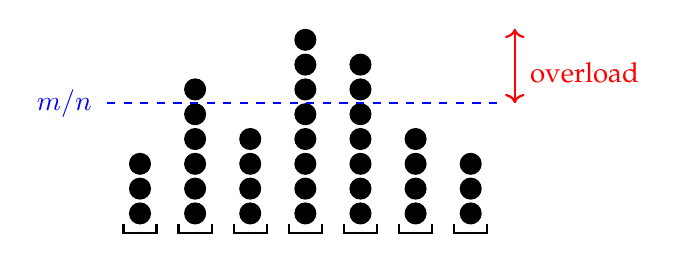
\begin{tikzpicture}[scale=0.7]
  % Define bin dimensions
  \def\binwidth{0.6}
  \def\ballradius{0.2}
  \def\binspacing{1.0}
  \def\avgheight{2.35}  % height for m/n line (top of 5th ball, m/n = 5)
  
  % Draw 7 bins as cups
  \def\sideheight{0.15}
  \foreach \i in {0,...,6} {
    \draw[thick] (\i*\binspacing, \sideheight) -- (\i*\binspacing, 0) -- (\i*\binspacing + \binwidth, 0) -- (\i*\binspacing + \binwidth, \sideheight);
  }
  
  % Add balls to bins (total = 35, so m/n = 5 exactly)
  % Bin 0: 3 balls
  \foreach \j in {1,2,3} {
    \fill[black] (0*\binspacing + \binwidth/2, \j*0.45 - 0.1) circle (\ballradius);
  }
  % Bin 1: 6 balls (above average)
  \foreach \j in {1,2,3,4,5,6} {
    \fill[black] (1*\binspacing + \binwidth/2, \j*0.45 - 0.1) circle (\ballradius);
  }
  % Bin 2: 4 balls
  \foreach \j in {1,2,3,4} {
    \fill[black] (2*\binspacing + \binwidth/2, \j*0.45 - 0.1) circle (\ballradius);
  }
  % Bin 3: 8 balls (the most overloaded bin!)
  \foreach \j in {1,2,3,4,5,6,7,8} {
    \fill[black] (3*\binspacing + \binwidth/2, \j*0.45 - 0.1) circle (\ballradius);
  }
  % Bin 4: 7 balls (above average)
  \foreach \j in {1,2,3,4,5,6,7} {
    \fill[black] (4*\binspacing + \binwidth/2, \j*0.45 - 0.1) circle (\ballradius);
  }
  % Bin 5: 4 balls
  \foreach \j in {1,2,3,4} {
    \fill[black] (5*\binspacing + \binwidth/2, \j*0.45 - 0.1) circle (\ballradius);
  }
  % Bin 6: 3 balls
  \foreach \j in {1,2,3} {
    \fill[black] (6*\binspacing + \binwidth/2, \j*0.45 - 0.1) circle (\ballradius);
  }
  
  % Dotted line at m/n (average height = 5 balls)
  \draw[dashed, thick, blue] (-0.3, \avgheight) -- (6*\binspacing + \binwidth + 0.3, \avgheight);
  \node[left, blue] at (-0.4, \avgheight) {$m/n$};
  
  % Overload bracket on the right side
  \draw[<->, thick, red] (6*\binspacing + \binwidth + 0.5, \avgheight) -- (6*\binspacing + \binwidth + 0.5, 8*0.45 - 0.1 + \ballradius);
  \node[right, red] at (6*\binspacing + \binwidth + 0.6, 2.9) {overload};
  
\end{tikzpicture}
\end{center}

\vspace{.3 cm}

  \textbf{Minimize Overload: } \\
  The amount by which the fullest bin exceeds $m/n$ is small. \pause

  \vspace{.4cm}

  \textbf{Minimize Recourse: } \\
  On any given insertion/deletion, the number of balls moved around is small.

\end{frame}

\begin{frame}{This Paper}

  \vspace{1 cm}

  \textbf{Question: }Does there exist a {\color{blue}history-independent} solution with small {\color{blue}recourse} and {\color{blue}overload}? \pause

  \vspace{1 cm}

  \textbf{Theorem: }There exists a {\color{blue}history-independent} solution with:
  \begin{itemize}
  \item {\color{blue}Overload $O(1)$}, with high probability.
  \item Expected {\color{blue}recourse $O(\log \log (m/n))$}.
  \end{itemize}
\end{frame}

\begin{frame}{What About Non-History-Independent Solutions?}

Lots of work on the insertion-only case. 
\\
{\color{gray} [Azar, Broder, Karlin and Upfal '94]
[Berenbrink, Czumaj, Steger, and V{\"o}cking '00][Dietzfelbinger and Weidling '07] 
[Frieze and Petti '18] $\ldots$} \pause 

\vspace{.2 cm}

But the fully dynamic case has remained largely open. \\
{\color{gray} [V{\"o}cking '99] [Dietzfelbinger and Weidling '07] [Bender, Conway, Farach-Colton, Kuszmaul, Tagliavini '21] [Bansal, Kuszmaul '22] $\ldots$} \pause

\vspace{.2 cm}

\textbf{Open Question: }\\
Is there a {\color{blue}fully dynamic} solution with {\color{blue}recourse $o(m/n)$} and {\color{blue}overload $O(1)$}? \pause

\vspace{.2 cm}

\textbf{Answer: }\\ 
Yes! We get {\color{blue}recourse $O(\log \log (m/n))$} and {\color{blue}overload $O(1)$}!

\end{frame}

\begin{frame}{This Paper}

  \vspace{1 cm}

  \textbf{Question: }Does there exist a {\color{blue}history-independent} solution with small {\color{blue}recourse} and {\color{blue}overload}? 

  \vspace{1 cm}

  \textbf{Theorem: }There exists a {\color{blue}history-independent} solution with:
  \begin{itemize}
  \item {\color{blue}Overload $O(1)$}, with high probability.
  \item Expected {\color{blue}recourse $O(\log \log (m/n))$}.
  \end{itemize}
\end{frame}

\begin{frame}{}

\vspace{2 cm}

\huge

\begin{center}
\textbf{Rest of Talk: } \\
Outlining a Solution with \\ Overload $O(\log \log n)$ \\ and Expected Recourse $O(m/n)$. 
\end{center}
\end{frame}

\begin{frame}{Warmup 1: The Single-Choice Strategy}

To insert a ball $x$, just put it in bin $h_1(x)$:

\begin{center}
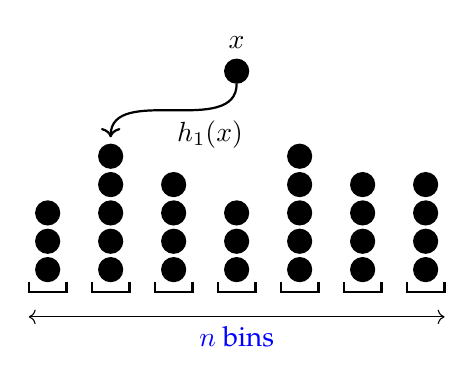
\begin{tikzpicture}[scale=0.8]
  % Define bin dimensions
  \def\binwidth{0.6}
  \def\ballradius{0.2}
  \def\binspacing{1.0}
  
  % Draw 7 bins as cups
  \def\sideheight{0.15}
  \foreach \i in {0,...,6} {
    \draw[thick] (\i*\binspacing, \sideheight) -- (\i*\binspacing, 0) -- (\i*\binspacing + \binwidth, 0) -- (\i*\binspacing + \binwidth, \sideheight);
  }
  
  % Add balls to bins (varying amounts)
  % Bin 0: 3 balls
  \foreach \j in {1,2,3} {
    \fill[black] (0*\binspacing + \binwidth/2, \j*0.45 - 0.1) circle (\ballradius);
  }
  % Bin 1: 5 balls
  \foreach \j in {1,2,3,4,5} {
    \fill[black] (1*\binspacing + \binwidth/2, \j*0.45 - 0.1) circle (\ballradius);
  }
  % Bin 2: 4 balls
  \foreach \j in {1,2,3,4} {
    \fill[black] (2*\binspacing + \binwidth/2, \j*0.45 - 0.1) circle (\ballradius);
  }
  % Bin 3: 3 balls
  \foreach \j in {1,2,3} {
    \fill[black] (3*\binspacing + \binwidth/2, \j*0.45 - 0.1) circle (\ballradius);
  }
  % Bin 4: 5 balls
  \foreach \j in {1,2,3,4,5} {
    \fill[black] (4*\binspacing + \binwidth/2, \j*0.45 - 0.1) circle (\ballradius);
  }
  % Bin 5: 4 balls
  \foreach \j in {1,2,3,4} {
    \fill[black] (5*\binspacing + \binwidth/2, \j*0.45 - 0.1) circle (\ballradius);
  }
  % Bin 6: 4 balls
  \foreach \j in {1,2,3,4} {
    \fill[black] (6*\binspacing + \binwidth/2, \j*0.45 - 0.1) circle (\ballradius);
  }
  
  % Ball x being inserted (centered above)
  \fill[black] (3*\binspacing + \binwidth/2, 3.5) circle (\ballradius);
  \node[above] at (3*\binspacing + \binwidth/2, 3.5 + \ballradius) {$x$};
  
  % Single arrow to h_1(x) - pointing to bin 1
  \draw[->, thick] (3*\binspacing + \binwidth/2, 3.5 - \ballradius) to[out=-90, in=90] (1*\binspacing + \binwidth/2, 5*0.45 + \ballradius);
  \node[right] at (2.2, 2.5) {$h_1(x)$};
  
  % Label: n bins
  \draw[<->] (0, -0.4) -- (6*\binspacing + \binwidth, -0.4);
  \node[below, blue] at (3*\binspacing + \binwidth/2, -0.4) {$n$ bins};
  
\end{tikzpicture}
\end{center}

\pause
\begin{itemize}
\item This is history-independent \hspace{0.3em}{\color{blue}\ding{51}} \pause
\item The recourse is 0 \hspace{0.3em}{\color{blue}\ding{51}} \pause
\item But... the overload is huge, roughly $\sqrt{m/n}$ \hspace{0.3em}{\color{red}\ding{55}}
\end{itemize}
\end{frame}

\begin{frame}{Warmup 2: Greedy Insertions}
  To insert a ball $x$, put it in the {\color{blue} emptier} of its choices:

\begin{center}
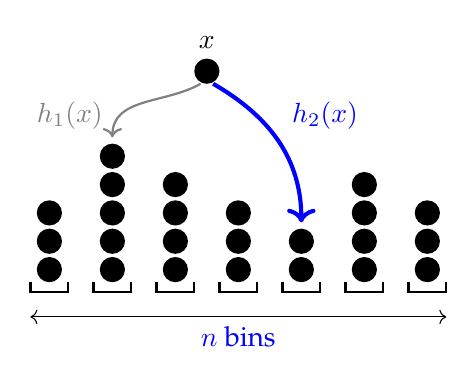
\begin{tikzpicture}[scale=0.8]
  % Define bin dimensions
  \def\binwidth{0.6}
  \def\ballradius{0.2}
  \def\binspacing{1.0}
  
  % Draw 7 bins as cups
  \def\sideheight{0.15}
  \foreach \i in {0,...,6} {
    \draw[thick] (\i*\binspacing, \sideheight) -- (\i*\binspacing, 0) -- (\i*\binspacing + \binwidth, 0) -- (\i*\binspacing + \binwidth, \sideheight);
  }
  
  % Add balls to bins
  % Bin 0: 3 balls
  \foreach \j in {1,2,3} {
    \fill[black] (0*\binspacing + \binwidth/2, \j*0.45 - 0.1) circle (\ballradius);
  }
  % Bin 1: 5 balls (one of x's choices - fuller)
  \foreach \j in {1,2,3,4,5} {
    \fill[black] (1*\binspacing + \binwidth/2, \j*0.45 - 0.1) circle (\ballradius);
  }
  % Bin 2: 4 balls
  \foreach \j in {1,2,3,4} {
    \fill[black] (2*\binspacing + \binwidth/2, \j*0.45 - 0.1) circle (\ballradius);
  }
  % Bin 3: 3 balls
  \foreach \j in {1,2,3} {
    \fill[black] (3*\binspacing + \binwidth/2, \j*0.45 - 0.1) circle (\ballradius);
  }
  % Bin 4: 2 balls (one of x's choices - emptier, x goes here!)
  \foreach \j in {1,2} {
    \fill[black] (4*\binspacing + \binwidth/2, \j*0.45 - 0.1) circle (\ballradius);
  }
  % Bin 5: 4 balls
  \foreach \j in {1,2,3,4} {
    \fill[black] (5*\binspacing + \binwidth/2, \j*0.45 - 0.1) circle (\ballradius);
  }
  % Bin 6: 3 balls
  \foreach \j in {1,2,3} {
    \fill[black] (6*\binspacing + \binwidth/2, \j*0.45 - 0.1) circle (\ballradius);
  }
  
  % Ball x being inserted (centered above)
  \fill[black] (2.5*\binspacing + \binwidth/2, 3.5) circle (\ballradius);
  \node[above] at (2.5*\binspacing + \binwidth/2, 3.5 + \ballradius) {$x$};
  
  % Two arrows to choices - bin 1 (fuller) and bin 4 (emptier)
  \draw[->, thick, gray] (2.5*\binspacing + \binwidth/2 - 0.1, 3.5 - \ballradius) to[out=-150, in=90] (1*\binspacing + \binwidth/2, 5*0.45 + \ballradius);
  \node[left, gray] at (1.3, 2.8) {$h_1(x)$};
  
  \draw[->, thick, blue, line width=1.5pt] (2.5*\binspacing + \binwidth/2 + 0.1, 3.5 - \ballradius) to[out=-30, in=90] (4*\binspacing + \binwidth/2, 2*0.45 + \ballradius);
  \node[right, blue] at (4.0, 2.8) {$h_2(x)$};
  
  % Label: n bins
  \draw[<->] (0, -0.4) -- (6*\binspacing + \binwidth, -0.4);
  \node[below, blue] at (3*\binspacing + \binwidth/2, -0.4) {$n$ bins};
  
\end{tikzpicture}
\end{center}



  \begin{itemize}
  \item This is \textbf{not} history-independent  \hspace{0.3em}{\color{red}\ding{55}} \pause
  \item The recourse is 0 \hspace{0.3em}{\color{blue}\ding{51}} \pause
  \item In the insertion-only case, the overload is $O(\log \log n)$ \hspace{0.3em}{\color{blue}\ding{51}} \\
  {\hfill \color{gray} [Azar, Broder, Karlin and Upfal '94]}
  \end{itemize}

  % \vspace{.4 cm}
  % \textbf{Interesting Fact: }In the dynamic case, overload remains open. \\
  % {\hfill \color{gray} [Bansal, Kuszmaul '22]}

\end{frame}

\begin{frame}{Turning Greedy into a History-Independent Solution}
\end{frame}

% ============== Two-World Slides ==============

% --- Frame 10 (PDF p10): initial two worlds, empty bins ---
\begin{frame}{Analyzing the Recourse}
\TopSeq
\TwoWorldFigure{ }{ }
\vfill
\hspace*{-1cm}\parbox{\dimexpr\textwidth+1cm}{%
\begin{itemize}
\item Two identical worlds, same insertion sequence
\item World 1 will later receive one extra ball $x^{\star}$
\end{itemize}
}
\end{frame}

% --- Frame 12 (PDF p12): x1 chooses among 2 bins ---
\begin{frame}{Analyzing the Recourse}
\TopSeq
\TwoWorldFigure{
  \node[circle,draw,minimum size=0.55cm,inner sep=0pt,RedBallStyle] (aL) at (-3.825,1.5) {$x_1$};
  \foreach \b in {1,3}{\draw[-{Stealth[length=2.5mm, width=1.8mm]},red!70!black,line width=0.7pt] (aL) -- (LT\b);}
}{
  \node[circle,draw,minimum size=0.55cm,inner sep=0pt,RedBallStyle] (aR) at (2.575,1.5) {$x_1$};
  \foreach \b in {1,3}{\draw[-{Stealth[length=2.5mm, width=1.8mm]},red!70!black,line width=0.7pt] (aR) -- (RT\b);}
}
\vfill
\hspace*{-1cm}\parbox{\dimexpr\textwidth+1cm}{%
\begin{itemize}
\item Two identical worlds, same insertion sequence
\item World 1 will later receive one extra ball $x^{\star}$
\end{itemize}
}
\end{frame}

% --- Frame 13 (PDF p13): x1 placed in bin 1 (both worlds) ---
\begin{frame}{Analyzing the Recourse}
\TopSeq
\TwoWorldFigure{
  \BallInBin{\xL}{1}{1}{RedBallStyle}{$x_1$}
}{
  \BallInBin{\xR}{1}{1}{RedBallStyle}{$x_1$}
}
\vfill
\hspace*{-1cm}\parbox{\dimexpr\textwidth+1cm}{%
\begin{itemize}
\item Two identical worlds, same insertion sequence
\item World 1 will later receive one extra ball $x^{\star}$
\end{itemize}
}
\end{frame}

% --- Frame 15 (PDF p15): x2 chooses among 2 bins (1 and 2) ---
\begin{frame}{Analyzing the Recourse}
\TopSeq
\TwoWorldFigure{
  \BallInBin{\xL}{1}{1}{}{}
  \node[circle,draw,minimum size=0.55cm,inner sep=0pt,RedBallStyle] (aL) at (-4.45,1.5) {$x_2$};
  \foreach \b in {1,2}{\draw[-{Stealth[length=2.5mm, width=1.8mm]},red!70!black,line width=0.7pt] (aL) -- (LT\b);}
}{
  \BallInBin{\xR}{1}{1}{}{}
  \node[circle,draw,minimum size=0.55cm,inner sep=0pt,RedBallStyle] (aR) at (1.95,1.5) {$x_2$};
  \foreach \b in {1,2}{\draw[-{Stealth[length=2.5mm, width=1.8mm]},red!70!black,line width=0.7pt] (aR) -- (RT\b);}
}
\vfill
\hspace*{-1cm}\parbox{\dimexpr\textwidth+1cm}{%
\begin{itemize}
\item Two identical worlds, same insertion sequence
\item World 1 will later receive one extra ball $x^{\star}$
\end{itemize}
}
\end{frame}

% --- Frame 16 (PDF p16): x2 placed in bin 2 (both worlds), plus prior ball in bin1 ---
\begin{frame}{Analyzing the Recourse}
\TopSeq
\TwoWorldFigure{
  \BallInBin{\xL}{1}{1}{}{}
  \BallInBin{\xL}{2}{1}{RedBallStyle}{$x_2$}
}{
  \BallInBin{\xR}{1}{1}{}{}
  \BallInBin{\xR}{2}{1}{RedBallStyle}{$x_2$}
}
\vfill
\hspace*{-1cm}\parbox{\dimexpr\textwidth+1cm}{%
\begin{itemize}
\item Two identical worlds, same insertion sequence
\item World 1 will later receive one extra ball $x^{\star}$
\end{itemize}
}
\end{frame}

% --- Frame 18 (PDF p18): x3 chooses among 2 bins (1 and 2) ---
\begin{frame}{Analyzing the Recourse}
\TopSeq
\TwoWorldFigure{
  \BallInBin{\xL}{1}{1}{}{}
  \BallInBin{\xL}{2}{1}{}{}
  \node[circle,draw,minimum size=0.55cm,inner sep=0pt,RedBallStyle] (aL) at (-4.45,1.5) {$x_3$};
  \foreach \b in {1,2}{\draw[-{Stealth[length=2.5mm, width=1.8mm]},red!70!black,line width=0.7pt] (aL) -- (LT\b);}
}{
  \BallInBin{\xR}{1}{1}{}{}
  \BallInBin{\xR}{2}{1}{}{}
  \node[circle,draw,minimum size=0.55cm,inner sep=0pt,RedBallStyle] (aR) at (1.95,1.5) {$x_3$};
  \foreach \b in {1,2}{\draw[-{Stealth[length=2.5mm, width=1.8mm]},red!70!black,line width=0.7pt] (aR) -- (RT\b);}
}
\vfill
\hspace*{-1cm}\parbox{\dimexpr\textwidth+1cm}{%
\begin{itemize}
\item Two identical worlds, same insertion sequence
\item World 1 will later receive one extra ball $x^{\star}$
\end{itemize}
}
\end{frame}

% --- Frame 19 (PDF p19): x3 placed in both worlds ---
\begin{frame}{Analyzing the Recourse}
\TopSeq
\TwoWorldFigure{
  \BallInBin{\xL}{1}{1}{}{}
  \BallInBin{\xL}{2}{1}{}{}
  \BallInBin{\xL}{2}{2}{RedBallStyle}{$x_3$}
}{
  \BallInBin{\xR}{1}{1}{}{}
  \BallInBin{\xR}{2}{1}{}{}
  \BallInBin{\xR}{2}{2}{RedBallStyle}{$x_3$}
}
\vfill
\hspace*{-1cm}\parbox{\dimexpr\textwidth+1cm}{%
\begin{itemize}
\item Two identical worlds, same insertion sequence
\item World 1 will later receive one extra ball $x^{\star}$
\end{itemize}
}
\end{frame}

% --- Frame 21 (PDF p21): x4 chooses among 2 bins (2 and 4) in both worlds ---
\begin{frame}{Analyzing the Recourse}
\TopSeq
\TwoWorldFigure{
  \BallInBin{\xL}{1}{1}{}{}
  \BallInBin{\xL}{2}{1}{}{}
  \BallInBin{\xL}{2}{2}{}{}
  \node[circle,draw,minimum size=0.55cm,inner sep=0pt,RedBallStyle] (aL) at (-2.575,1.5) {$x_4$};
  \foreach \b in {2,4}{\draw[-{Stealth[length=2.5mm, width=1.8mm]},red!70!black,line width=0.7pt] (aL) -- (LT\b);}
}{
  \BallInBin{\xR}{1}{1}{}{}
  \BallInBin{\xR}{2}{1}{}{}
  \BallInBin{\xR}{2}{2}{}{}
  \node[circle,draw,minimum size=0.55cm,inner sep=0pt,RedBallStyle] (aR) at (3.825,1.5) {$x_4$};
  \foreach \b in {2,4}{\draw[-{Stealth[length=2.5mm, width=1.8mm]},red!70!black,line width=0.7pt] (aR) -- (RT\b);}
}
\vfill
\hspace*{-1cm}\parbox{\dimexpr\textwidth+1cm}{%
\begin{itemize}
\item Two identical worlds, same insertion sequence
\item World 1 will later receive one extra ball $x^{\star}$
\end{itemize}
}
\end{frame}

% --- Frame 22 (PDF p22): x4 placed in bin4 in both worlds ---
\begin{frame}{Analyzing the Recourse}
\TopSeq
\TwoWorldFigure{
  \BallInBin{\xL}{1}{1}{}{}
  \BallInBin{\xL}{2}{1}{}{}
  \BallInBin{\xL}{2}{2}{}{}
  \BallInBin{\xL}{4}{1}{RedBallStyle}{$x_4$}
}{
  \BallInBin{\xR}{1}{1}{}{}
  \BallInBin{\xR}{2}{1}{}{}
  \BallInBin{\xR}{2}{2}{}{}
  \BallInBin{\xR}{4}{1}{RedBallStyle}{$x_4$}
}
\vfill
\hspace*{-1cm}\parbox{\dimexpr\textwidth+1cm}{%
\begin{itemize}
\item Two identical worlds, same insertion sequence
\item World 1 will later receive one extra ball $x^{\star}$
\end{itemize}
}
\end{frame}

% --- Frame 24 (PDF p24): x* (blue outline) chooses between bins (3 and 4) in world1 ---
\begin{frame}{Analyzing the Recourse}
\TopSeq
\TwoWorldFigure{
  \BallInBin{\xL}{1}{1}{}{}
  \BallInBin{\xL}{2}{1}{}{}
  \BallInBin{\xL}{2}{2}{}{}
  \BallInBin{\xL}{4}{1}{}{}
}{
  \BallInBin{\xR}{1}{1}{}{}
  \BallInBin{\xR}{2}{1}{}{}
  \BallInBin{\xR}{2}{2}{}{}
  \BallInBin{\xR}{4}{1}{}{}
  \node[circle,draw,minimum size=0.55cm,inner sep=0pt,BlueOutlineStyle] (bR) at (3.825,1.5) {$x^{\star}$};
  \foreach \bb in {2,4}{\draw[-{Stealth[length=2.5mm, width=1.8mm]},blue!70!black,line width=0.7pt] (bR) -- (RT\bb);}
}
\vfill
\hspace*{-1cm}\parbox{\dimexpr\textwidth+1cm}{%
\begin{itemize}
\item $x^{\star}$ arrives only in World 1
\end{itemize}
}
\end{frame}

% --- Frame 25 (PDF p25): x* placed (blue outline, labeled) in world1 bin4 top ---
\begin{frame}{Analyzing the Recourse}
\TopSeq
\TwoWorldFigure{
  \BallInBin{\xL}{1}{1}{}{}
  \BallInBin{\xL}{2}{1}{}{}
  \BallInBin{\xL}{2}{2}{}{}
  \BallInBin{\xL}{4}{1}{}{}
}{
  \BallInBin{\xR}{1}{1}{}{}
  \BallInBin{\xR}{2}{1}{}{}
  \BallInBin{\xR}{2}{2}{}{}
  \BallInBin{\xR}{4}{1}{}{}
  \BallInBin{\xR}{4}{2}{BlueOutlineStyle}{$x^{\star}$}
}
\vfill
\hspace*{-1cm}\parbox{\dimexpr\textwidth+1cm}{%
\begin{itemize}
\item $x^{\star}$ arrives only in World 1
\end{itemize}
}
\end{frame}

% --- Frame 26: Question about divergence ---
\begin{frame}{Analyzing the Recourse}
\TopSeq
\TwoWorldFigure{
  \BallInBin{\xL}{1}{1}{}{}
  \BallInBin{\xL}{2}{1}{}{}
  \BallInBin{\xL}{2}{2}{}{}
  \BallInBin{\xL}{4}{1}{}{}
}{
  \BallInBin{\xR}{1}{1}{}{}
  \BallInBin{\xR}{2}{1}{}{}
  \BallInBin{\xR}{2}{2}{}{}
  \BallInBin{\xR}{4}{1}{}{}
  \BallInBin{\xR}{4}{2}{BlueFillStyle}{}
}
\vfill
\hspace*{-0.5cm}\parbox{\dimexpr\textwidth+0.5cm}{%
\textbf{Question:} How do subsequent insertions differ between the two worlds?
}
\end{frame}

% --- Frame 27 (PDF p27): future insertions: option 1 (No recourse) ---
\begin{frame}{Analyzing the Recourse}
\TopSeq
\TwoWorldFigure{
  \BallInBin{\xL}{1}{1}{}{}
  \BallInBin{\xL}{2}{1}{}{}
  \BallInBin{\xL}{2}{2}{}{}
  \BallInBin{\xL}{4}{1}{}{}
}{
  \BallInBin{\xR}{1}{1}{}{}
  \BallInBin{\xR}{2}{1}{}{}
  \BallInBin{\xR}{2}{2}{}{}
  \BallInBin{\xR}{4}{1}{}{}
  \BallInBin{\xR}{4}{2}{BlueFillStyle}{}
}
\vfill
\hspace*{-0.5cm}\parbox{\dimexpr\textwidth+0.5cm}{%
Future insertions will experience either: \pause
\begin{enumerate}
\item No recourse
\end{enumerate}
}
\end{frame}

% --- Frame 28 (PDF p28): x5 chooses among 2 bins (1 and 3) ---
\begin{frame}{Analyzing the Recourse}
\TopSeq
\TwoWorldFigure{
  \BallInBin{\xL}{1}{1}{}{}
  \BallInBin{\xL}{2}{1}{}{}
  \BallInBin{\xL}{2}{2}{}{}
  \BallInBin{\xL}{4}{1}{}{}
  \node[circle,draw,minimum size=0.55cm,inner sep=0pt,RedBallStyle] (aL) at (-3.825,1.5) {$x_5$};
  \foreach \b in {1,3}{\draw[-{Stealth[length=2.5mm, width=1.8mm]},red!70!black,line width=0.7pt] (aL) -- (LT\b);}
}{
  \BallInBin{\xR}{1}{1}{}{}
  \BallInBin{\xR}{2}{1}{}{}
  \BallInBin{\xR}{2}{2}{}{}
  \BallInBin{\xR}{4}{1}{}{}
  \BallInBin{\xR}{4}{2}{BlueFillStyle}{}
  \node[circle,draw,minimum size=0.55cm,inner sep=0pt,RedBallStyle] (aR) at (2.575,1.5) {$x_5$};
  \foreach \b in {1,3}{\draw[-{Stealth[length=2.5mm, width=1.8mm]},red!70!black,line width=0.7pt] (aR) -- (RT\b);}
}
\vfill
\hspace*{-0.5cm}\parbox{\dimexpr\textwidth+0.5cm}{%
Future insertions will experience either:
\begin{enumerate}
\item No recourse
\end{enumerate}
}
\end{frame}

% --- Frame 29 (PDF p29): x5 placed in bin3 (both worlds) ---
\begin{frame}{Analyzing the Recourse}
\TopSeq
\TwoWorldFigure{
  \BallInBin{\xL}{1}{1}{}{}
  \BallInBin{\xL}{2}{1}{}{}
  \BallInBin{\xL}{2}{2}{}{}
  \BallInBin{\xL}{3}{1}{RedBallStyle}{$x_5$}
  \BallInBin{\xL}{4}{1}{}{}
}{
  \BallInBin{\xR}{1}{1}{}{}
  \BallInBin{\xR}{2}{1}{}{}
  \BallInBin{\xR}{2}{2}{}{}
  \BallInBin{\xR}{3}{1}{RedBallStyle}{$x_5$}
  \BallInBin{\xR}{4}{1}{}{}
  \BallInBin{\xR}{4}{2}{BlueFillStyle}{}
}
\vfill
\hspace*{-0.5cm}\parbox{\dimexpr\textwidth+0.5cm}{%
Future insertions will experience either:
\begin{enumerate}
\item No recourse
\end{enumerate}
}
\end{frame}

% --- Frame 31 (PDF p31): x6 chooses among 2 bins (1 and 3) ---
\begin{frame}{Analyzing the Recourse}
\TopSeq
\TwoWorldFigure{
  \BallInBin{\xL}{1}{1}{}{}
  \BallInBin{\xL}{2}{1}{}{}
  \BallInBin{\xL}{2}{2}{}{}
  \BallInBin{\xL}{3}{1}{}{}
  \BallInBin{\xL}{4}{1}{}{}
  \node[circle,draw,minimum size=0.55cm,inner sep=0pt,RedBallStyle] (aL) at (-3.825,1.5) {$x_6$};
  \foreach \b in {1,3}{\draw[-{Stealth[length=2.5mm, width=1.8mm]},red!70!black,line width=0.7pt] (aL) -- (LT\b);}
}{
  \BallInBin{\xR}{1}{1}{}{}
  \BallInBin{\xR}{2}{1}{}{}
  \BallInBin{\xR}{2}{2}{}{}
  \BallInBin{\xR}{3}{1}{}{}
  \BallInBin{\xR}{4}{1}{}{}
  \BallInBin{\xR}{4}{2}{BlueFillStyle}{}
  \node[circle,draw,minimum size=0.55cm,inner sep=0pt,RedBallStyle] (aR) at (2.575,1.5) {$x_6$};
  \foreach \b in {1,3}{\draw[-{Stealth[length=2.5mm, width=1.8mm]},red!70!black,line width=0.7pt] (aR) -- (RT\b);}
}
\vfill
\hspace*{-0.5cm}\parbox{\dimexpr\textwidth+0.5cm}{%
Future insertions will experience either:
\begin{enumerate}
\item No recourse
\end{enumerate}
}
\end{frame}

% --- Frame 32 (PDF p32): x6 placed in bin3 (level 2) ---
\begin{frame}{Analyzing the Recourse}
\TopSeq
\TwoWorldFigure{
  \BallInBin{\xL}{1}{1}{}{}
  \BallInBin{\xL}{2}{1}{}{}
  \BallInBin{\xL}{2}{2}{}{}
  \BallInBin{\xL}{3}{1}{}{}
  \BallInBin{\xL}{3}{2}{RedBallStyle}{$x_6$}
  \BallInBin{\xL}{4}{1}{}{}
}{
  \BallInBin{\xR}{1}{1}{}{}
  \BallInBin{\xR}{2}{1}{}{}
  \BallInBin{\xR}{2}{2}{}{}
  \BallInBin{\xR}{3}{1}{}{}
  \BallInBin{\xR}{3}{2}{RedBallStyle}{$x_6$}
  \BallInBin{\xR}{4}{1}{}{}
  \BallInBin{\xR}{4}{2}{BlueFillStyle}{}
}
\vfill
\hspace*{-0.5cm}\parbox{\dimexpr\textwidth+0.5cm}{%
Future insertions will experience either:
\begin{enumerate}
\item No recourse
\end{enumerate}
}
\end{frame}

% --- Frame 34 (PDF p34): x7 chooses among 2 bins (2 and 3) ---
\begin{frame}{Analyzing the Recourse}
\TopSeq
\TwoWorldFigure{
  \BallInBin{\xL}{1}{1}{}{}
  \BallInBin{\xL}{2}{1}{}{}
  \BallInBin{\xL}{2}{2}{}{}
  \BallInBin{\xL}{3}{1}{}{}
  \BallInBin{\xL}{3}{2}{}{}
  \BallInBin{\xL}{4}{1}{}{}
  \node[circle,draw,minimum size=0.55cm,inner sep=0pt,RedBallStyle] (aL) at (-3.2,1.5) {$x_7$};
  \foreach \b in {2,3}{\draw[-{Stealth[length=2.5mm, width=1.8mm]},red!70!black,line width=0.7pt] (aL) -- (LT\b);}
}{
  \BallInBin{\xR}{1}{1}{}{}
  \BallInBin{\xR}{2}{1}{}{}
  \BallInBin{\xR}{2}{2}{}{}
  \BallInBin{\xR}{3}{1}{}{}
  \BallInBin{\xR}{3}{2}{}{}
  \BallInBin{\xR}{4}{1}{}{}
  \BallInBin{\xR}{4}{2}{BlueFillStyle}{}
  \node[circle,draw,minimum size=0.55cm,inner sep=0pt,RedBallStyle] (aR) at (3.2,1.5) {$x_7$};
  \foreach \b in {2,3}{\draw[-{Stealth[length=2.5mm, width=1.8mm]},red!70!black,line width=0.7pt] (aR) -- (RT\b);}
}
\vfill
\hspace*{-0.5cm}\parbox{\dimexpr\textwidth+0.5cm}{%
Future insertions will experience either:
\begin{enumerate}
\item No recourse
\end{enumerate}
}
\end{frame}

% --- Frame 35 (PDF p35): x7 placed in bin3 (level 3) ---
\begin{frame}{Analyzing the Recourse}
\TopSeq
\TwoWorldFigure{
  \BallInBin{\xL}{1}{1}{}{}
  \BallInBin{\xL}{2}{1}{}{}
  \BallInBin{\xL}{2}{2}{}{}
  \BallInBin{\xL}{3}{1}{}{}
  \BallInBin{\xL}{3}{2}{}{}
  \BallInBin{\xL}{3}{3}{RedBallStyle}{$x_7$}
  \BallInBin{\xL}{4}{1}{}{}
}{
  \BallInBin{\xR}{1}{1}{}{}
  \BallInBin{\xR}{2}{1}{}{}
  \BallInBin{\xR}{2}{2}{}{}
  \BallInBin{\xR}{3}{1}{}{}
  \BallInBin{\xR}{3}{2}{}{}
  \BallInBin{\xR}{3}{3}{RedBallStyle}{$x_7$}
  \BallInBin{\xR}{4}{1}{}{}
  \BallInBin{\xR}{4}{2}{BlueFillStyle}{}
}
\vfill
\hspace*{-0.5cm}\parbox{\dimexpr\textwidth+0.5cm}{%
Future insertions will experience either:
\begin{enumerate}
\item No recourse
\end{enumerate}
}
\end{frame}

% --- Frame 36: x7 greyed, add option 2 (Recourse) ---
\begin{frame}{Analyzing the Recourse}
\TopSeq
\TwoWorldFigure{
  \BallInBin{\xL}{1}{1}{}{}
  \BallInBin{\xL}{2}{1}{}{}
  \BallInBin{\xL}{2}{2}{}{}
  \BallInBin{\xL}{3}{1}{}{}
  \BallInBin{\xL}{3}{2}{}{}
  \BallInBin{\xL}{3}{3}{}{}
  \BallInBin{\xL}{4}{1}{}{}
}{
  \BallInBin{\xR}{1}{1}{}{}
  \BallInBin{\xR}{2}{1}{}{}
  \BallInBin{\xR}{2}{2}{}{}
  \BallInBin{\xR}{3}{1}{}{}
  \BallInBin{\xR}{3}{2}{}{}
  \BallInBin{\xR}{3}{3}{}{}
  \BallInBin{\xR}{4}{1}{}{}
  \BallInBin{\xR}{4}{2}{BlueFillStyle}{}
}
\vfill
\hspace*{-0.5cm}\parbox{\dimexpr\textwidth+0.5cm}{%
Future insertions will experience either:
\begin{enumerate}
\item No recourse
\item Recourse
\end{enumerate}
}
\end{frame}

% --- Frame 37: x8 chooses between bins 1 and 4 ---
\begin{frame}{Analyzing the Recourse}
\TopSeq
\TwoWorldFigure{
  \BallInBin{\xL}{1}{1}{}{}
  \BallInBin{\xL}{2}{1}{}{}
  \BallInBin{\xL}{2}{2}{}{}
  \BallInBin{\xL}{3}{1}{}{}
  \BallInBin{\xL}{3}{2}{}{}
  \BallInBin{\xL}{3}{3}{}{}
  \BallInBin{\xL}{4}{1}{}{}
  \node[circle,draw,minimum size=0.55cm,inner sep=0pt,RedBallStyle] (aL) at (-3.2,1.5) {$x_8$};
  \foreach \b in {1,4}{\draw[-{Stealth[length=2.5mm, width=1.8mm]},red!70!black,line width=0.7pt] (aL) -- (LT\b);}
}{
  \BallInBin{\xR}{1}{1}{}{}
  \BallInBin{\xR}{2}{1}{}{}
  \BallInBin{\xR}{2}{2}{}{}
  \BallInBin{\xR}{3}{1}{}{}
  \BallInBin{\xR}{3}{2}{}{}
  \BallInBin{\xR}{3}{3}{}{}
  \BallInBin{\xR}{4}{1}{}{}
  \BallInBin{\xR}{4}{2}{BlueFillStyle}{}
  \node[circle,draw,minimum size=0.55cm,inner sep=0pt,RedBallStyle] (aR) at (3.2,1.5) {$x_8$};
  \foreach \b in {1,4}{\draw[-{Stealth[length=2.5mm, width=1.8mm]},red!70!black,line width=0.7pt] (aR) -- (RT\b);}
}
\vfill
\hspace*{-0.5cm}\parbox{\dimexpr\textwidth+0.5cm}{%
Future insertions will experience either:
\begin{enumerate}
\item No recourse
\item Recourse
\end{enumerate}
}
\end{frame}

% --- Frame 38: x8 placed in bin 4 (world 0) and bin 1 (world 1) ---
\begin{frame}{Analyzing the Recourse}
\TopSeq
\TwoWorldFigure{
  \BallInBin{\xL}{1}{1}{}{}
  \BallInBin{\xL}{2}{1}{}{}
  \BallInBin{\xL}{2}{2}{}{}
  \BallInBin{\xL}{3}{1}{}{}
  \BallInBin{\xL}{3}{2}{}{}
  \BallInBin{\xL}{3}{3}{}{}
  \BallInBin{\xL}{4}{1}{}{}
  \BallInBin{\xL}{4}{2}{RedBallStyle}{$x_8$}
}{
  \BallInBin{\xR}{1}{1}{}{}
  \BallInBin{\xR}{1}{2}{RedBallStyle}{$x_8$}
  \BallInBin{\xR}{2}{1}{}{}
  \BallInBin{\xR}{2}{2}{}{}
  \BallInBin{\xR}{3}{1}{}{}
  \BallInBin{\xR}{3}{2}{}{}
  \BallInBin{\xR}{3}{3}{}{}
  \BallInBin{\xR}{4}{1}{}{}
  \BallInBin{\xR}{4}{2}{BlueFillStyle}{}
}
\vfill
\hspace*{-0.5cm}\parbox{\dimexpr\textwidth+0.5cm}{%
Future insertions will experience either:
\begin{enumerate}
\item No recourse
\item Recourse
\end{enumerate}
}
\end{frame}

% --- Frame 39: all grey, top ball in bin 1 world 1 is blue ---
\begin{frame}{Analyzing the Recourse}
\TopSeq
\TwoWorldFigure{
  \BallInBin{\xL}{1}{1}{}{}
  \BallInBin{\xL}{2}{1}{}{}
  \BallInBin{\xL}{2}{2}{}{}
  \BallInBin{\xL}{3}{1}{}{}
  \BallInBin{\xL}{3}{2}{}{}
  \BallInBin{\xL}{3}{3}{}{}
  \BallInBin{\xL}{4}{1}{}{}
  \BallInBin{\xL}{4}{2}{}{}
}{
  \BallInBin{\xR}{1}{1}{}{}
  \BallInBin{\xR}{1}{2}{BlueFillStyle}{}
  \BallInBin{\xR}{2}{1}{}{}
  \BallInBin{\xR}{2}{2}{}{}
  \BallInBin{\xR}{3}{1}{}{}
  \BallInBin{\xR}{3}{2}{}{}
  \BallInBin{\xR}{3}{3}{}{}
  \BallInBin{\xR}{4}{1}{}{}
  \BallInBin{\xR}{4}{2}{}{}
}
\vfill
\hspace*{-0.5cm}\parbox{\dimexpr\textwidth+0.5cm}{%
Future insertions will experience either:
\begin{enumerate}
\item No recourse
\item Recourse
\end{enumerate}
}
\end{frame}

% --- Frame 40: x9 chooses between bins 1 and 2 ---
\begin{frame}{Analyzing the Recourse}
\TopSeq
\TwoWorldFigure{
  \BallInBin{\xL}{1}{1}{}{}
  \BallInBin{\xL}{2}{1}{}{}
  \BallInBin{\xL}{2}{2}{}{}
  \BallInBin{\xL}{3}{1}{}{}
  \BallInBin{\xL}{3}{2}{}{}
  \BallInBin{\xL}{3}{3}{}{}
  \BallInBin{\xL}{4}{1}{}{}
  \BallInBin{\xL}{4}{2}{}{}
  \node[circle,draw,minimum size=0.55cm,inner sep=0pt,RedBallStyle] (aL) at (-4.45,1.5) {$x_9$};
  \foreach \b in {1,2}{\draw[-{Stealth[length=2.5mm, width=1.8mm]},red!70!black,line width=0.7pt] (aL) -- (LT\b);}
}{
  \BallInBin{\xR}{1}{1}{}{}
  \BallInBin{\xR}{1}{2}{BlueFillStyle}{}
  \BallInBin{\xR}{2}{1}{}{}
  \BallInBin{\xR}{2}{2}{}{}
  \BallInBin{\xR}{3}{1}{}{}
  \BallInBin{\xR}{3}{2}{}{}
  \BallInBin{\xR}{3}{3}{}{}
  \BallInBin{\xR}{4}{1}{}{}
  \BallInBin{\xR}{4}{2}{}{}
  \node[circle,draw,minimum size=0.55cm,inner sep=0pt,RedBallStyle] (aR) at (1.95,1.5) {$x_9$};
  \foreach \b in {1,2}{\draw[-{Stealth[length=2.5mm, width=1.8mm]},red!70!black,line width=0.7pt] (aR) -- (RT\b);}
}
\vfill
\hspace*{-0.5cm}\parbox{\dimexpr\textwidth+0.5cm}{%
Future insertions will experience either:
\begin{enumerate}
\item No recourse
\item Recourse
\end{enumerate}
}
\end{frame}

% --- Frame 41: x9 placed in bin 1 (world 0) and bin 2 (world 1) ---
\begin{frame}{Analyzing the Recourse}
\TopSeq
\TwoWorldFigure{
  \BallInBin{\xL}{1}{1}{}{}
  \BallInBin{\xL}{1}{2}{RedBallStyle}{$x_9$}
  \BallInBin{\xL}{2}{1}{}{}
  \BallInBin{\xL}{2}{2}{}{}
  \BallInBin{\xL}{3}{1}{}{}
  \BallInBin{\xL}{3}{2}{}{}
  \BallInBin{\xL}{3}{3}{}{}
  \BallInBin{\xL}{4}{1}{}{}
  \BallInBin{\xL}{4}{2}{}{}
}{
  \BallInBin{\xR}{1}{1}{}{}
  \BallInBin{\xR}{1}{2}{BlueFillStyle}{}
  \BallInBin{\xR}{2}{1}{}{}
  \BallInBin{\xR}{2}{2}{}{}
  \BallInBin{\xR}{2}{3}{RedBallStyle}{$x_9$}
  \BallInBin{\xR}{3}{1}{}{}
  \BallInBin{\xR}{3}{2}{}{}
  \BallInBin{\xR}{3}{3}{}{}
  \BallInBin{\xR}{4}{1}{}{}
  \BallInBin{\xR}{4}{2}{}{}
}
\vfill
\hspace*{-0.5cm}\parbox{\dimexpr\textwidth+0.5cm}{%
Future insertions will experience either:
\begin{enumerate}
\item No recourse
\item Recourse
\end{enumerate}
}
\end{frame}

% --- Frame 42: all grey, top ball in bin 2 world 1 is blue ---
\begin{frame}{Analyzing the Recourse}
\TopSeq
\TwoWorldFigure{
  \BallInBin{\xL}{1}{1}{}{}
  \BallInBin{\xL}{1}{2}{}{}
  \BallInBin{\xL}{2}{1}{}{}
  \BallInBin{\xL}{2}{2}{}{}
  \BallInBin{\xL}{3}{1}{}{}
  \BallInBin{\xL}{3}{2}{}{}
  \BallInBin{\xL}{3}{3}{}{}
  \BallInBin{\xL}{4}{1}{}{}
  \BallInBin{\xL}{4}{2}{}{}
}{
  \BallInBin{\xR}{1}{1}{}{}
  \BallInBin{\xR}{1}{2}{}{}
  \BallInBin{\xR}{2}{1}{}{}
  \BallInBin{\xR}{2}{2}{}{}
  \BallInBin{\xR}{2}{3}{BlueFillStyle}{}
  \BallInBin{\xR}{3}{1}{}{}
  \BallInBin{\xR}{3}{2}{}{}
  \BallInBin{\xR}{3}{3}{}{}
  \BallInBin{\xR}{4}{1}{}{}
  \BallInBin{\xR}{4}{2}{}{}
}
\vfill
\hspace*{-0.5cm}\parbox{\dimexpr\textwidth+0.5cm}{%
Future insertions will experience either:
\begin{enumerate}
\item No recourse
\item Recourse
\end{enumerate}
}
\end{frame}

% --- Frame 43: Two key observations ---
\begin{frame}{Analyzing the Recourse}
\TopSeq
\TwoWorldFigure{
  \BallInBin{\xL}{1}{1}{}{}
  \BallInBin{\xL}{1}{2}{}{}
  \BallInBin{\xL}{2}{1}{}{}
  \BallInBin{\xL}{2}{2}{}{}
  \BallInBin{\xL}{3}{1}{}{}
  \BallInBin{\xL}{3}{2}{}{}
  \BallInBin{\xL}{3}{3}{}{}
  \BallInBin{\xL}{4}{1}{}{}
  \BallInBin{\xL}{4}{2}{}{}
}{
  \BallInBin{\xR}{1}{1}{}{}
  \BallInBin{\xR}{1}{2}{}{}
  \BallInBin{\xR}{2}{1}{}{}
  \BallInBin{\xR}{2}{2}{}{}
  \BallInBin{\xR}{2}{3}{BlueFillStyle}{}
  \BallInBin{\xR}{3}{1}{}{}
  \BallInBin{\xR}{3}{2}{}{}
  \BallInBin{\xR}{3}{3}{}{}
  \BallInBin{\xR}{4}{1}{}{}
  \BallInBin{\xR}{4}{2}{}{}
}
\vfill
\hspace*{-0.5cm}\parbox{\dimexpr\textwidth+0.5cm}{%
Two key observations: \pause
\begin{enumerate}
\item There's always one special bin with an extra ball \pause
\item Recourse requires the special bin as one of the two choices
\end{enumerate}
}
\end{frame}

% --- Frame 44: Probability calculation ---
\begin{frame}{Analyzing the Recourse}
\TopSeq
\TwoWorldFigure{
  \BallInBin{\xL}{1}{1}{}{}
  \BallInBin{\xL}{1}{2}{}{}
  \BallInBin{\xL}{2}{1}{}{}
  \BallInBin{\xL}{2}{2}{}{}
  \BallInBin{\xL}{3}{1}{}{}
  \BallInBin{\xL}{3}{2}{}{}
  \BallInBin{\xL}{3}{3}{}{}
  \BallInBin{\xL}{4}{1}{}{}
  \BallInBin{\xL}{4}{2}{}{}
}{
  \BallInBin{\xR}{1}{1}{}{}
  \BallInBin{\xR}{1}{2}{}{}
  \BallInBin{\xR}{2}{1}{}{}
  \BallInBin{\xR}{2}{2}{}{}
  \BallInBin{\xR}{2}{3}{BlueFillStyle}{}
  \BallInBin{\xR}{3}{1}{}{}
  \BallInBin{\xR}{3}{2}{}{}
  \BallInBin{\xR}{3}{3}{}{}
  \BallInBin{\xR}{4}{1}{}{}
  \BallInBin{\xR}{4}{2}{}{}
}
\vfill
\hspace*{-0.5cm}\parbox{\dimexpr\textwidth+0.5cm}{%
\[
\Pr[\text{ball } x_i \text{ incurs recourse}] = O(1/n)
\]
\pause
\[
\implies \mathbb{E}[\text{total recourse}] = \sum_{i} \Pr[\text{ball } x_i \text{ incurs recourse}] = O(m/n)
\]
}
\end{frame}

\end{document}